\chapter{Introduction}

%\section{Household robots in general}
More and more robots appear in everyday life. Automatic vacuum cleaners and floor washers are getting widespread, as the technology is becoming cheaper and better. The vacuum cleaners have matured to a level, where they are been considered for saving man-hours in the elderly care sector.\\

\noindent
Outside the walls of our homes lays the next weekly hurdle: Mowing the lawn. A known way to handle this, is to pay the neighbour's teenager to do it. Unfortunately they grow up and move out, leaving the lawns in the residential neighbourhoods behind.\\ 

\noindent
Luckily engineers have stepped in, and provided a more long-term solution: Robotic lawn mowers.

\section{Robotic lawn mowers}
Several manufacturers of electrical gardening machines have started selling robotic lawn mowers in the recent years. In general they use one of two strategies when cutting the lawn:
\begin{itemize}
	\item Random direction mowers
	\item Parallel line mowers
\end{itemize}

\noindent
Mowers using the random direction strategy will drive in a straight line until a guard wire or an obstacle is detected. They will then turn in a random direction, and continue. See \figref{fig:randomcut}

\begin{figure}[H]
\centering
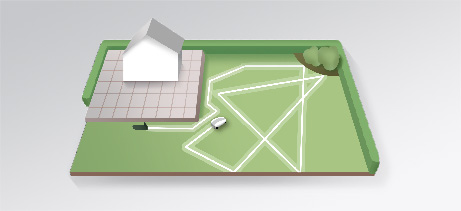
\includegraphics[scale=0.8]{figures/noLogiCut.jpg} 
\label{fig:randomcut}
\caption{Random cut system [source:Bosch]} 
\end{figure}

\noindent
When the battery is nearly discharged, the mower will follow the guard wire back to the base station for recharging.\\

\noindent
Parallel line mowers use a more intelligent control algorithm to optimize the mowing. After an initial learning run, following the guard wire around the lawn to be mowed, it will map the lawn, and cut in parallel lines, see \figref{fig:logicut}. The advantage of this strategy efficiency, as the lawn mower will not run over the same spots more than once. According to Bosch, a given lawn can be mowed up to 30\% faster with their Logicut system.
%% TODO: Insert source
 

\begin{figure}[H]
\centering
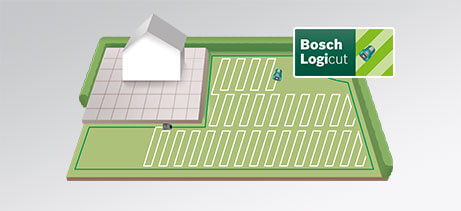
\includegraphics[scale=0.8]{figures/logicut.jpg} 
\label{fig:logicut}
\caption{Bosch Logicut system [source:Bosch]} 
\end{figure}

\noindent
Common for both systems is the guard wire, which has to be placed around the lawn and anywhere the lawn mower is not allowed to go, like flower beds, swimming pools, etc. \\

\noindent
This brings us to the problem with existing products.

\section{Problems with existing robotic lawn mowers}
All commercially available robotic lawn mowers requires a guard wire placed around the lawn. This can either be placed at the surface, and be held in place by pegs, or dug down below the surface. The guard wire must be routed around flower beds, etc. as well, see \figref{fig:robomow}

 
\begin{figure}[H]
\centering
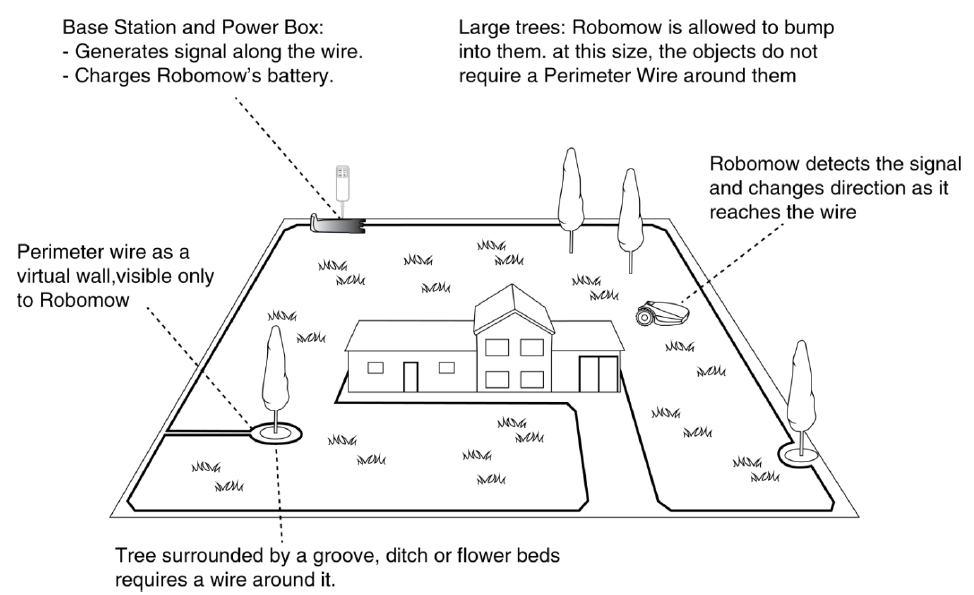
\includegraphics[scale=0.6]{figures/robomow.png} 
\label{fig:robomow}
\caption{Guard wire installation [source:Robomow]} 
\end{figure}
\noindent

The use of the guard wire for guiding the mower back to the charging station presents another potential problem: in a garden with many restricted areas, the guard wire could get very long. This could therefore make the journey home long, compared to a more direct route. This again uses more battery power, that instead could have been used for actually mowing the lawn.\\

\noindent
This will be the motivation for the project: to avoid the work routing a wire around the garden, and as a bonus get more work done on a battery charge, by not wasting power following the wire home.\\

\noindent
Then, the question is : what other solutions could we use to get the lawn mower to go where we want it to go? \\
One first step could be to keep track of where it is in real-time.

%-- Section : GoT introductory presentation --%
\section{The Games on Track (GoT) system}
We were provided with the \emph{Games on Track GT-Position} system as a start to be able to figure out the lawn mower position in space.\\

\noindent
It is composed of four different parts both hardware and software :
%% TODO : Add reference to http://www.gamesontrack.co.uk/pages/webside.asp?articleGuid=64556
\begin{itemize}
	\item The tracked module, which emits ultra-sound waves. It should be placed on our lawn mower itself, so that the emitting cell is not obstructed by anything.
	\item Some beacons or receivers, placed all around the place the lawn mower will move in. Depending on the terrain, we can use from 2 to more than 20 of these : the more we place, the more accuracy we can get to fight against any ambieznt noise.
	\item The central system which gathers information about the distance of the tracked module to each beacon and transmits it to the computer via USB in regular intervals.
	\item The GoT software aggregates the received positions thoughout time and can be used to draw a map of the terrain (the lawn) and send every needed information to a third-party (our) piece of software.
\end{itemize}
GoT was firstly designed for train modeling but it is easily adaptable for any use of position tracking and seems a good choice, at first, for our autonomous lawn mower.\\
But, why wouldn't we use a satellite based positioning system ?

%-- Section : Satellite vs GoT --%
\section{Satellite based positioning systems vs GoT}
The reasons why satellite positioning system won't be used in our project are mainly related to accuracy and energy consumption.\\

\noindent
Indeed, these kinds of system like GPS or GLONASS would require a dedicated chip to put on the final system. The problem then would be the lack of precision under a few meters (around 2 or 3 meters in ideal situations for the best chips). \\
%% TODO : Add reference to "A Review of GLONASS" Miller, 2000 & http://www.gps.gov/systems/gps/performance/accuracy/ %

\noindent
Moreover, this kind of system implies slow communications with different distant satellites at the same time. Therefore, the energy consumption would quickly rise, thus reducing the lawn mower autonomy, which is not desirable.

\section{Potential consumer expectations}
The design of a product has no real value if no one is interested in using it. Thus, choices made during this project have to be made in accordance with the final user's expectations.\\

\noindent
For instance, we need to keep in mind some considerations regarding the autonomy of the vehicle (both in energy and for the navigation), but also towards the overall cost \fxwarning{insert price approximation here}. Even though, the GoT system itself has a cost beyond anything a normal customer would pay for a lawn mower, it appears, at first, as a good solution for us in terms of accuracy and energy consumption compared to GPS-like systems which are also quite expensive \fxwarning{insert price approximation here - not so true actually}. \\

\noindent
For an improvement, we could consider replacing it with a similar solution as it is only a simple brick of the whole system. \fxnote{This sentence should be perhaps moved to a dedicated part of the report}\\

\noindent
These are the types of preliminary considerations that will influence our design process for an autonomous lawn mower.